% Chapter Template

\chapter{Ensayos y Resultados} % Main chapter title

\label{Chapter4} % Change X to a consecutive number; for referencing this chapter elsewhere, use \ref{ChapterX}

%----------------------------------------------------------------------------------------

La idea de esta sección es explicar cómo se hicieron los ensayos, qué resultados se obtuvieron y analizarlos.

\section{Ensayos de caja negra}

\section{Hardware}

\begin{figure}[h]
	\centering
	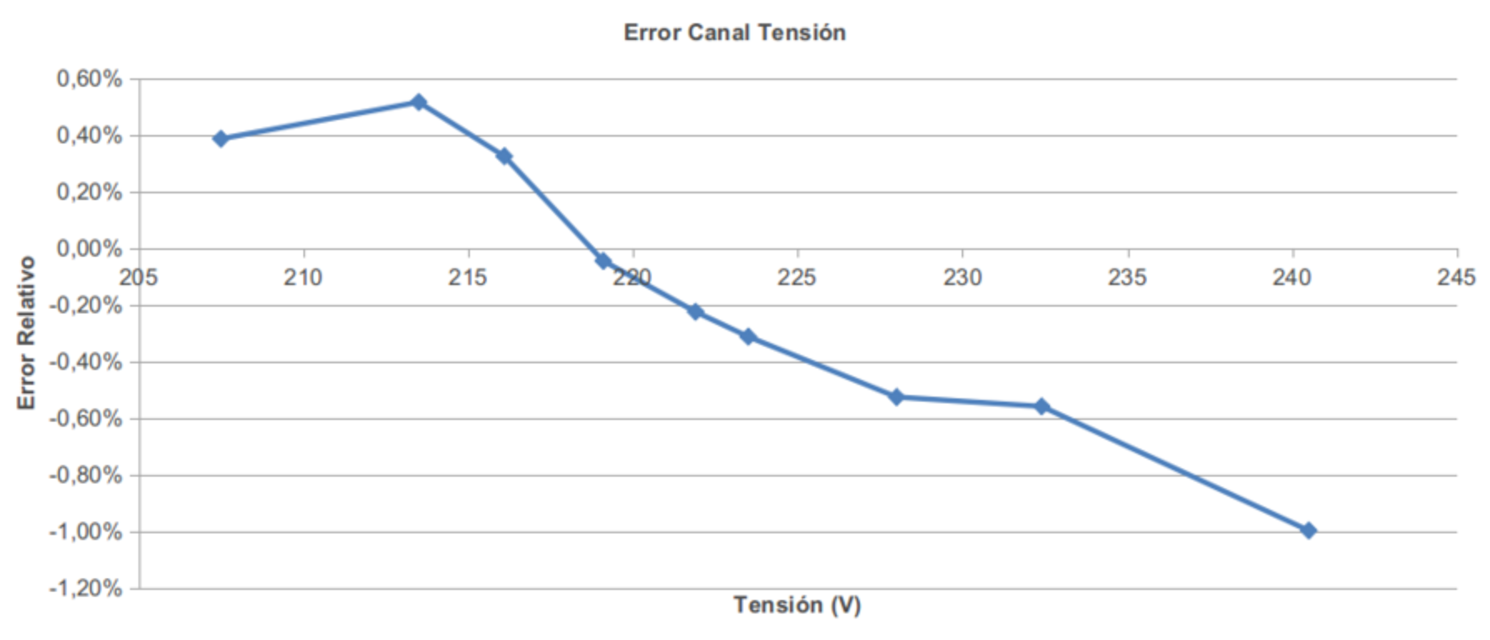
\includegraphics[width=10cm]{./Figures/4_1_1_error_canal_tension.pdf}
	\caption{Error relativo en el canal de tensión.}
	\label{fig:error_canal_tensión}
\end{figure}

\begin{figure}[h]
	\centering
	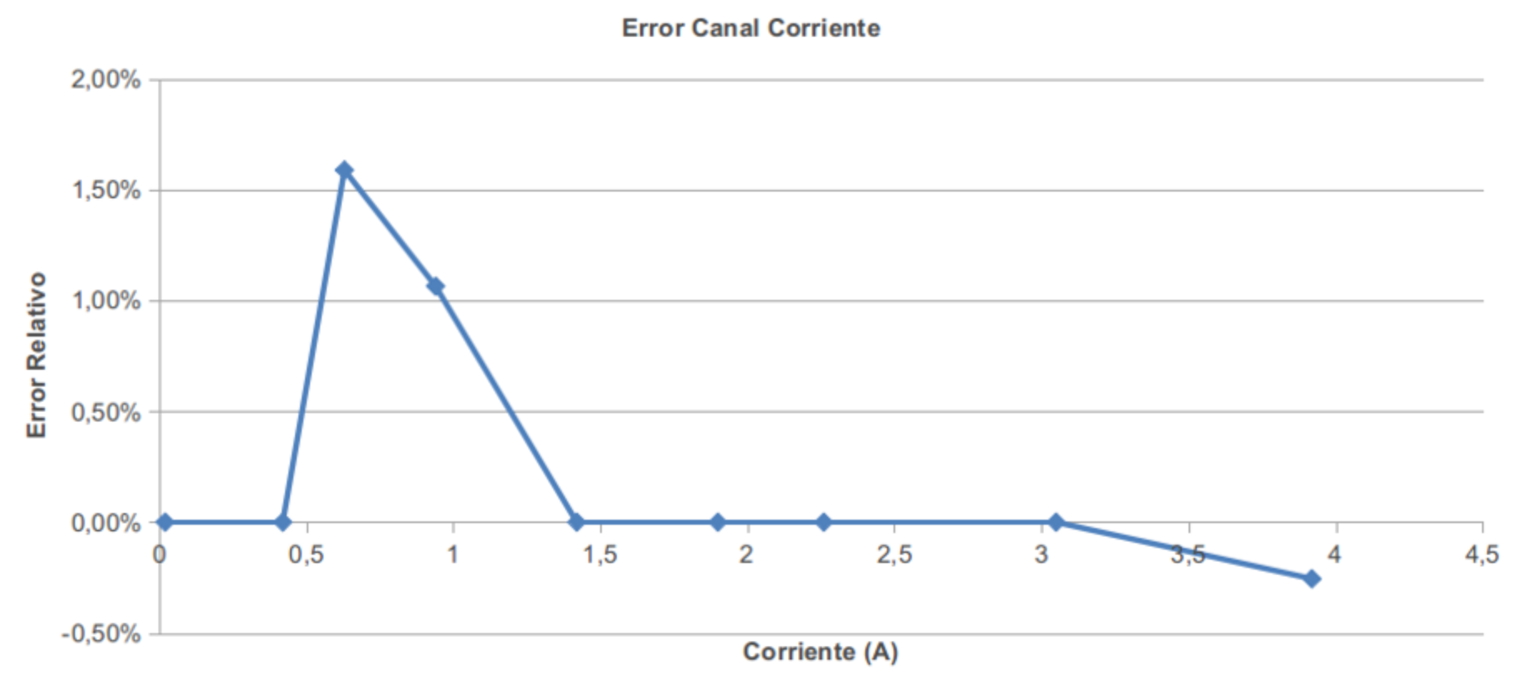
\includegraphics[width=10cm]{./Figures/4_1_1_error_canal_corriente.pdf}
	\caption{Error relativo en el canal de corriente.}
	\label{fig:error_canal_corriente}
\end{figure}

\section{Firmware}
\label{sec:validacion_firmware}

\begin{figure}[h]
	\centering
	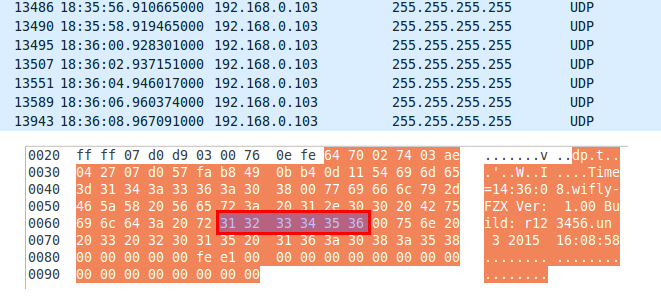
\includegraphics[width=12cm]{./Figures/4_1_2_mensajes_udp.png}
	\caption{Mensajes UDP periódicos recibidos de un Smart Plug, utilizados para identificarlo dentro de la red WiFi.}
	\label{fig:mensajes_udp}
\end{figure}

\begin{figure}[h]
	\centering
	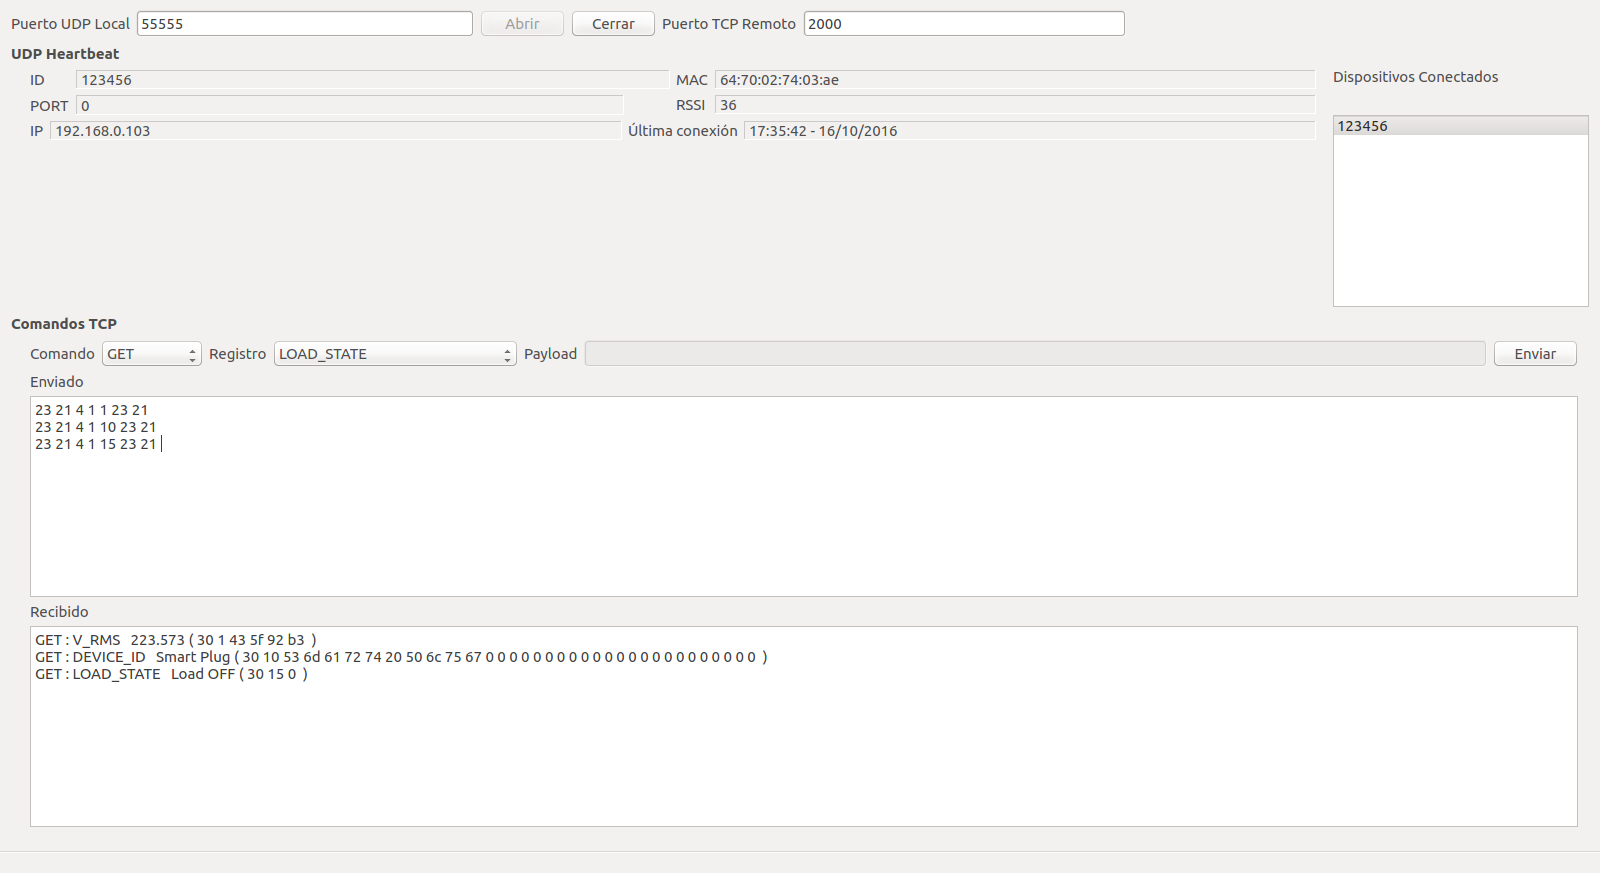
\includegraphics[width=14cm]{./Figures/4_1_2_simulador_tcp.png}
	\caption{Captura del software desarrollado que permite generar todos los comandos propuestos en el protocolo de comunicación.}
	\label{fig:simulador_tcp}
\end{figure}

\section{Aplicación móvil}

